\documentclass{article}


\usepackage{arxiv}
\usepackage{mypackage}

\usepackage[utf8]{inputenc} % allow utf-8 input
\usepackage[T1]{fontenc}    % use 8-bit T1 fonts
\usepackage{hyperref}       % hyperlinks
\usepackage{url}            % simple URL typesetting
\usepackage{booktabs}       % professional-quality tables
\usepackage{amsfonts}       % blackboard math symbols
\usepackage{nicefrac}       % compact symbols for 1/2, etc.
\usepackage{microtype}      % microtypography
\usepackage{lipsum}

\makeatletter
\def\and{%
  \end{tabular}%
  \begin{tabular}[t]{c}}%
\def\@fnsymbol#1{\ensuremath{\ifcase#1\or a\or b\or c\or
   d\or e\or f\or g\or h\or i\else\@ctrerr\fi}}
\makeatother

\makeatletter % `@' now normal "letter"
\@addtoreset{equation}{section}
\makeatother  % `@' is restored as "non-letter"
\renewcommand\theequation{\oldstylenums{\thesection}.\oldstylenums{\arabic{equation}}}

\begin{document}
\title{CSCI-610 paper: Deduce an NFA from the black box by using machine learning method}

\author{Zheng Li}
\maketitle

% \tableofcontents
% \newpage

% ==============================================================
\begin{abstract}
    In the present paper, we introduce some related paper that works on reducing the automata structure of the black box by learning its inputs and outputs firstly. 
    By researching these papers,  we propose a novel method that can deduce an NFA with structure as simple as possible from the black box. The related program and the ideal is 100\% original. 
\end{abstract}

% ==============================================================
\section{Introduction}
The learning techniques are usually employed for inferring a formal model such as finite state automaton (FA) or finite state machine (FSM) (also called transducer) of a system whose internal behaviour is implicit and unknown. It has become widespread in the domain of formal verification (e.g., \cite{peled1999black,groce2002adaptive,cobleigh2003learning,chaki2008verification}).
For instance, if we have permission to use a given software, but cannot view its source code. We can record the outputs of this software by trying a series of different inputs, then construct corresponding automata by using this technique. 


However, such general problems are usually extremely difficult\cite{pacharoen2013active} so that we need to limit their range. Therefore, in the present paper, we discuss the method that can deduce an NFA with the simplest structure by learning the corresponding dataset. Fig. (\ref{fig: architecture}) demonstrates my idea, we can convert this problem to the typical question: \textbf{Generate the simplest automata that only accept a given series string.} If we require the automata to be a DFA, the question will be easy. However, such a solution may not be the best, because DFA usually has more finite states than its equivalent NFA. As we know, we can easily convert an NFA to a DFA by computing the closure, but hard to reduce the number of states by converting a DFA to an NFA. Although we can use the Myphill-Nerode Theorem\cite{nerode1958linear} to minimize DFA, we are going to explore the possibility of using machine learning methods. In addition, the program is open source \href{https://github.com/ZhengLiCS/CSCI-610}{\color{cyan}https://github.com/ZhengLiCS/CSCI-610}.

\section{Description of the idea}
As we mentioned before, we need to convert the problem into a string recognition problem. Fig.(\ref{fig: architecture}) shows the method, we each pair of input and output of the black box, we convert 
them into a binary vector with fixed length respectively. The map should be a bijection, it implies that different input/output will match different binary vector.

Assuming the input vector in the space $\{ 0, 1 \}^m$ and output vector in the space $\{ T, F \}^n$, then when the calculation process of the black box is equivalent to the recognition process of $2^n$ NFAs(each NFA ouput one component of the output vector). By enumerating all the inputs cases, we will obtain all recognized results, and all the NFAs will be certain. Therefore the example in the dataset consists of two parts, the input binary string and ouput binary vector, the corresponding target is the certained NFAs.

So far we have the dataset, then consider training a model that can output a series of NFAs when inputting a pair of binary string and vector. If the cardinality $2^n$ is not very large, the Random Forest\cite{ho1995random} should be the best model, because it can predict results precisely. If the cardinality $2^n$ is extremely large, the Deep Neural Network\cite{goodfellow2016deep} should be the best model, because it can process the high-dimensional features.

\begin{figure}[H]
    \centering
    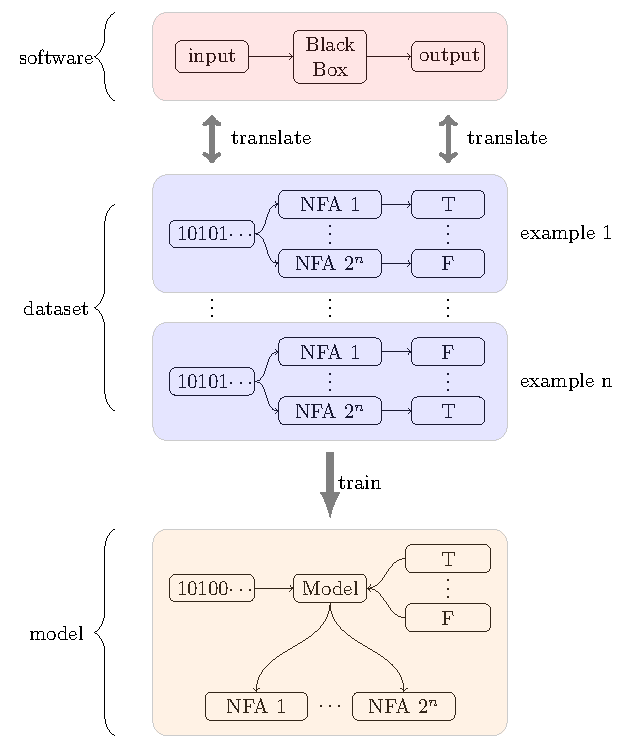
\includegraphics[width=0.5\linewidth]{src/architecture.pdf}
    \caption{
        \protect\tikz\protect\node[draw, fill=red!50, opacity=0.2] at (0, 0) { }; Software,
        \protect\tikz\protect\node[draw, fill=blue!50, opacity=0.2] at (0, 0) { }; Examples in dataset,
        \protect\tikz\protect\node[draw, fill=orange!50, opacity=0.2] at (0, 0) { }; Machine learning model,
    }
    \label{fig: architecture}
\end{figure}

If using the Deep Neural Network, we can train the model by using the following SGD algorithm, where the $(Q', \Sigma', \delta', q', F') = f(\boldsymbol{x}; \boldsymbol{\theta})$ is the predict NFA and 
\begin{equation*}
    \| f(\boldsymbol{x}; \boldsymbol{\theta}) - (Q, \Sigma, \delta, q, F) \| = 
    \| Q - Q' \| + \| \Sigma - \Sigma' \| + \| \delta - \delta' \| + \| q - q' \| + \| F - F' \| 
\end{equation*}
\begin{figure}[H]
    \centering
    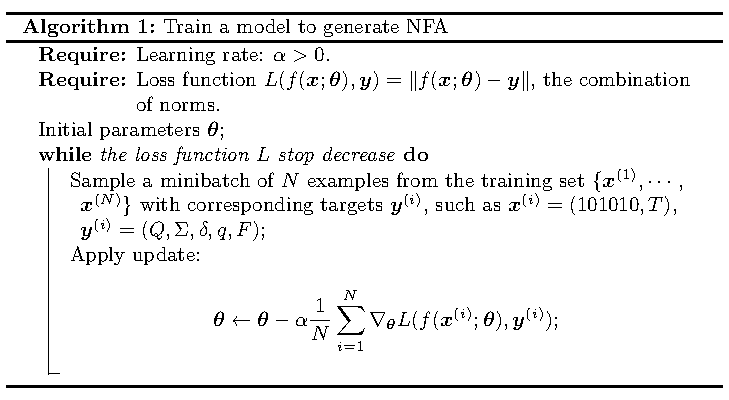
\includegraphics[width=0.75\linewidth]{src/train_loop.pdf}
    % \caption{ }
    \label{alg: train loop}
\end{figure}

\section{Analysis and evaluations}
The address of our open-source program is \href{https://github.com/ZhengLiCS/CSCI-610}{\color{cyan}https://github.com/ZhengLiCS/CSCI-610}, we list some results of the demo experiment below
\begin{figure}[H]
    \centering
    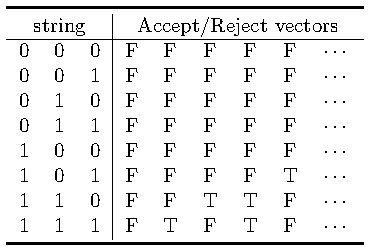
\includegraphics[width=0.75\linewidth]{src/experiments.pdf}
    % \caption{ }
    \label{tab: experiments}
\end{figure}
For the first instance, the black box read strings ["000", "001", ..., "111"] one by one, then output ["F", "F", "F", "F", "F", "F", "F", "F"] one by one. The model will predict the following NFA
\begin{itemize}
    \item states: $[q_0, q_1]$
    \item alphabet: $[0, 1]$
    \item start state: $q_0$
    \item accept states: $\{ q_1 \}$
    \item transition function: 
    \begin{tabular}{l|lll}
              & 0             & 1             & $\varepsilon$ \\ \hline
        $q_0$ & $\varnothing$ & $\{ q_1 \}$   & $\varnothing$ \\   
        $q_1$ & $\varnothing$ & $\varnothing$ & $\varnothing$ \\  
    \end{tabular}
\end{itemize}
For the second instance, the black box read strings ["000", "001", ..., "111"] one by one, then output ["F", "F", "F", "F", "F", "F", "F", "T"] one by one. The model will predict the following NFA
\begin{itemize}
    \item states: $[q_0, q_1]$
    \item alphabet: $[0, 1]$
    \item start state: $q_0$
    \item accept states: $\{ q_1 \}$
    \item transition function: 
    \begin{tabular}{l|lll}
              & 0             & 1             & $\varepsilon$ \\ \hline
        $q_0$ & $\varnothing$ & $\varnothing$ & $\{ q_1 \}$ \\   
        $q_1$ & $\varnothing$ & $\{ q_1 \}$   & $\varnothing$ \\  
    \end{tabular}
\end{itemize}
For the third instance, the black box read strings ["000", "001", ..., "111"] one by one, then output ["F", "F", "F", "F", "F", "F", "T", "F"] one by one. The model will predict the following NFA
\begin{itemize}
    \item states: $[q_0, q_1]$
    \item alphabet: $[0, 1]$
    \item start state: $q_0$
    \item accept states: $\{ q_0 \}$
    \item transition function: 
    \begin{tabular}{l|lll}
              & 0             & 1             & $\varepsilon$ \\ \hline
        $q_0$ & $\varnothing$ & $\{ q_1 \}$   & $\varnothing$ \\   
        $q_1$ & $\{ q_0 \}$   & $\{ q_1 \}$   & $\varnothing$ \\  
    \end{tabular}
\end{itemize}
For the fourth instance, the black box read strings ["000", "001", ..., "111"] one by one, then output ["F", "F", "F", "F", "F", "F", "T", "T"] one by one. The model will predict the following NFA
\begin{itemize}
    \item states: $[q_0, q_1]$
    \item alphabet: $[0, 1]$
    \item start state: $q_0$
    \item accept states: $\{ q_0 \}$
    \item transition function: 
    \begin{tabular}{l|lll}
              & 0             & 1             & $\varepsilon$ \\ \hline
        $q_0$ & $\varnothing$ & $\{ q_1 \}$   & $\varnothing$ \\   
        $q_1$ & $\{ q_0 \}$   & $\{ q_0, q_1 \}$   & $\varnothing$ \\  
    \end{tabular}
\end{itemize}
For the fifth instance, the black box read strings ["000", "001", ..., "111"] one by one, then output ["F", "F", "F", "F", "F", "T", "F", "F"] one by one. The model will predict the following NFA
\begin{itemize}
    \item states: $[q_0, q_1]$
    \item alphabet: $[0, 1]$
    \item start state: $q_0$
    \item accept states: $\{ q_0 \}$
    \item transition function: 
    \begin{tabular}{l|lll}
              & 0             & 1             & $\varepsilon$ \\ \hline
        $q_0$ & $\varnothing$ & $\{ q_1 \}$   & $\varnothing$ \\   
        $q_1$ & $\{ q_1 \}$   & $\{ q_0 \}$   & $\varnothing$ \\  
    \end{tabular}
\end{itemize}


\section{Conclusion}
From experiments, we are sure the machine learning method works. However, it is not suitable for the case that the string length is extremely large. Why? denote the cardinality of finite states set as $n_{states}$, the cardinality of alphabet as $n_{alphabet}$ and the length of string as $n_{length}$, then there are totally $2^{n_{states}} \times (n_{alphabet}^{n_{states}})^{(n_{alphabet} + 1) \times n_{states}}$ kinds of NFAs that we have to learn! It's too large! Therefore, if the string length is very large, we recommend using the traditional methods.



\bibliographystyle{unsrt}  
\bibliography{references} 


\end{document}


% Thank you, Zhang. This is Zheng Li. Now let me demonstrate some examples. 

% Our framework consists of three directories and three python files. The utils.py is the collection of various parent classes that we mentioned before. The script covid.py and nyc_accident.py are the collections of child classes of the two datasets in our report respectively. The directory src contains the corresponding datasets and other geography JSON files. The directory cache contains some temporary files that can accelerate the online computation. And we save our models in the directory logs.


% ------------------ unit testing ----------------------
% For each child class in the our program, we designed the corresponding unit testing method to make sure the software is working correctly. Ok, let start the demo.


% ------------------ Visulization ----------------------
% Now we are running the MatplotlibTimeSeriesVisualtion. As you can see, in the child class, for a new dataset, we don't have to rewrite the method.

% When we move the mouse, the canvas will highlight the top-5 curves and decrease the opacity of other curves. There are two widgets in the GUI, the set of radio buttons and the slider. 

% Let's turn to the MatplotlibTimeFreeVisualtion. The pie chart shows the top-10 locations and we can change the attributes by moving the slider. This is the box plot and this is the histogram.


% ------------------ Visulization ----------------------
% We demonstrate five data mining tasks in this unit testing method.
%     * Using the Decission tree to predict the category. Here is the Visulization of decision tree, we limit the depth as 16 and number of leaf nodes as 300.
%     * Using the Random Forest to predict values of various attributes. Then using the cross validation method to selcted the best models. Finally evaluate the models by computing its R2 score.
%     * Using the Random Forest to predict the values of various attributes. Then using the cross validation method to selcted the best models. Finally evaluate the models by computing its R2 score.
%     * And the association analysis and the sequential pattern mining. the program will display all solutions in the terminal.
